% #######################################
% ########### FILL THESE IN #############
% #######################################
\def\mytitle{MATRICES}
\def\mykeywords{}
\def\myauthor{GOWTHAMI MANDAVA}
\def\contact{gowthamimandava999@gmail.com}
\def\mymodule{ Future Wireless Communication(FWC22012)}
% #######################################
% #### YOU DON'T NEED TO TOUCH BELOW ####
% #######################################
\newcommand{\myvec}[1]{\ensuremath{\begin{pmatrix}#1\end{pmatrix}}}
\let\vec\mathbf
\providecommand{\pr}[1]{\ensuremath{\Pr\left(#1\right)}}
\providecommand{\qfunc}[1]{\ensuremath{Q\left(#1\right)}}
\providecommand{\sbrak}[1]{\ensuremath{{}\left[#1\right]}}
\providecommand{\lsbrak}[1]{\ensuremath{{}\left[#1\right.}}
\providecommand{\rsbrak}[1]{\ensuremath{{}\left.#1\right]}}
\providecommand{\brak}[1]{\ensuremath{\left(#1\right)}}
\providecommand{\lbrak}[1]{\ensuremath{\left(#1\right.}}
\providecommand{\rbrak}[1]{\ensuremath{\left.#1\right)}}
\providecommand{\cbrak}[1]{\ensuremath{\left\{#1\right\}}}
\providecommand{\lcbrak}[1]{\ensuremath{\left\{#1\right.}}
\providecommand{\rcbrak}[1]{\ensuremath{\left.#1\right\}}}
\documentclass[10pt, a4paper]{article}
\usepackage[a4paper,outer=1.5cm,inner=1.5cm,top=1.75cm,bottom=1.5cm]{geometry}
\twocolumn
\usepackage{circuitikz}
\usepackage{amsmath,bm}
\usepackage{amsthm}
\usepackage{mathtools}
\usepackage{amsfonts}
\usepackage{amssymb}
\usepackage{graphicx}
\graphicspath{{./images/}}
%colour our links, remove weird boxes
\usepackage[colorlinks,linkcolor={black},citecolor={blue!80!black},urlcolor={blue!80!black}]{hyperref}
%Stop indentation on new paragraphs
\usepackage[parfill]{parskip}
%% Arial-like font
\usepackage{lmodern}
\renewcommand*\familydefault{\sfdefault}
%Napier logo top right
\usepackage{watermark}
%Lorem Ipusm dolor please don't leave any in you final report ;)
\usepackage{karnaugh-map} 
\usepackage{tabularx}
\usepackage{lipsum}
\usepackage{xcolor}
\usepackage{listings}
%give us the Capital H that we all know and love
\usepackage{float}
%tone down the line spacing after section titles
\usepackage{titlesec}
%Cool maths printing
\usepackage{amsmath}
%PseudoCode
\usepackage{algorithm2e}

\titlespacing{\subsection}{0pt}{\parskip}{-3pt}
\titlespacing{\subsubsection}{0pt}{\parskip}{-\parskip}
\titlespacing{\paragraph}{0pt}{\parskip}{\parskip}
\newcommand{\figuremacro}[5]{
    \begin{figure}[#1]
        \centering
        \includegraphics[width=#5\columnwidth]{#2}
        \caption[#3]{\textbf{#3}#4}
        \label{fig:#2}
    \end{figure}
}


 \lstset{
frame=single, 
breaklines=true,
columns=fullflexible
}

\thiswatermark{\centering \put(1,-110){
\includegraphics[scale=0.05]{IIT_logo.jpg}} }
\title{\mytitle}
\author{\myauthor\hspace{1em}\\\contact\\IITH\hspace{0.5em}-\hspace{0.5em}\mymodule}
\date{}
\hypersetup{pdfauthor=\myauthor,pdftitle=\mytitle,pdfkeywords=\mykeywords}
\sloppy
% #######################################
% ########### START FROM HERE ###########
% #######################################
\begin{document}
 \maketitle
 \tableofcontents
  \Large\section{Problem}
 \textbf{Q}.The circle passing through tha point (_1,0) and touching the y-axis at (0,2) also passes through the point
  \section{Solution}
 \begin{center}
     Given,
      the point (-1,0)  is passing through the circle 
      \\ and the circle is touching the y-axis at(0,2)
       \\ so the eqation of circle using matrices can be written as,
       \begin{align}       
\textbf{x}^{\top}\textbf{V}\textbf{x}+2\textbf{x}\textbf{U}^{\top}+f=0
\end{align}
Let $\textbf{A}$=$\myvec{-1\\0}$ and $\textbf{B}$=$\myvec{0\\2}$ and  $\textbf{m}$=$\myvec{0\\1}$
\begin{equation}
        \textbf{A}\textbf{A}^{\top} + 2\textbf{u}^{\top}\textbf{A} + f = 0
\end{equation}
\begin{equation}
        ||{\textbf{A}}||^2 + 2\textbf{A}^{\top} \textbf{u} + f = 0
\end{equation}
\begin{equation}
        \myvec{2\textbf{A}^{\top} & 1}\myvec{\textbf{u} \\ f} =-||\textbf{A}||^2
\end{equation}
\begin{equation}
        \textbf{B}\textbf{B}^{\top} + 2\textbf{u}^{\top}\textbf{B} + f = 0
\end{equation}
\begin{equation}
        \myvec{2\textbf{B}^{\top} & 1}\myvec{\textbf{u} \\ f} = -||{\textbf{B}}||^2
\end{equation}
The equation of the tangent is
\begin{equation}
        \textbf{m}^{\top} (\textbf{V}q + \textbf{u}) = 0
\end{equation}
\begin{equation}
        \textbf{m}^T\textbf{A} +\textbf{m}^T\textbf{u} = 0
\end{equation}
\begin{equation}
         \textbf{m}^{\top}\textbf{u} = -\textbf{m}^{\top}\textbf{A}
\end{equation}
from equations (4),(6) and (9),we can write as
\begin{equation}
        \myvec{\textbf{m}^{\top} & 0 \\ 2\textbf{A}^{\top} & 1 \\ 2\textbf{B}^{\top} & 1}\myvec{\textbf{u} \\ f} = \myvec{-\textbf{m}^T\textbf{A} \\ -||{\textbf{A}}||^2 \\ -||{\textbf{B}}||^2}
\end{equation}
\myvec{0&1&0 \\0 & 4& 1 \\ -2 & 0 & 1} \myvec{\textbf{u}\\f}=\myvec{-2\\-4\\-1} \\
solving the equations
\begin{center}
$\myvec{0&1&0&-2 \\0 & 4& 1 & -4 \\ -2 & 0 & 1 & -1 } \xrightarrow[]{R_1 \leftarrow R_3 }$\\
$\myvec{-2&0&1&-1 \\0 & 4 & 1 & -4 \\ 0 & 1 & 0 & -2 } \xrightarrow[]{R_1 \leftarrow R_1/-2 } $\\
$\myvec{1&0&-1/2&1/2 \\0 & 4 & 1 & -4 \\ 0 & 1 & 0 & -2 } \xrightarrow[]{R_2 \leftarrow  R_2/4 }$\\
$\myvec{1&0&-1/2&1/2 \\0 & 1 & 1/4 & -1 \\ 0 & 1 & 0 & -2 } \xrightarrow[]{R_3 \leftarrow R_3- R_2 }$\\
$\myvec{1&0&-1/2&1/2 \\0 & 1 & 1/4 & -1 \\ 0 & 0 & -1/4 & -1 } \xrightarrow[]{R_3 \leftarrow R_3*-4 }$\\
$\myvec{1&0&1/2&1/2 \\0 & 1 & 1/4 & -1 \\ 0 & 0 & 1 & 4 }$\xrightarrow[]{R_2 \leftarrow R_2-1/4R_3 }$
$\myvec{1&0&-1/2&1/2 \\0 & 1 & 0 & -2 \\ 0 & 0 & 1 & 4 } \xrightarrow[]{R_1 \leftarrow R_1+1/2R_3 }$\\
$\myvec{1&0&0&5/2 \\0 & 1 & 0 & -2 \\ 0 & 0 & 1 & 4 }\\
\end{center}
By solving the above equations\\\\ $\textbf{u} =\myvec{5/2 \\ -2}$\\
c=-\textbf{u}\\
c=\myvec{-5/2&2} is the center of circle\\
f=4
\\as y-axis touches the circle the radius of the circle becomes 
\\r=5/2
 \\by substituing given options in the above equation (-4,0) satifies the equation 
 \\ the third point which is passing through given circle is (-4,0)             
 \section{Plot}
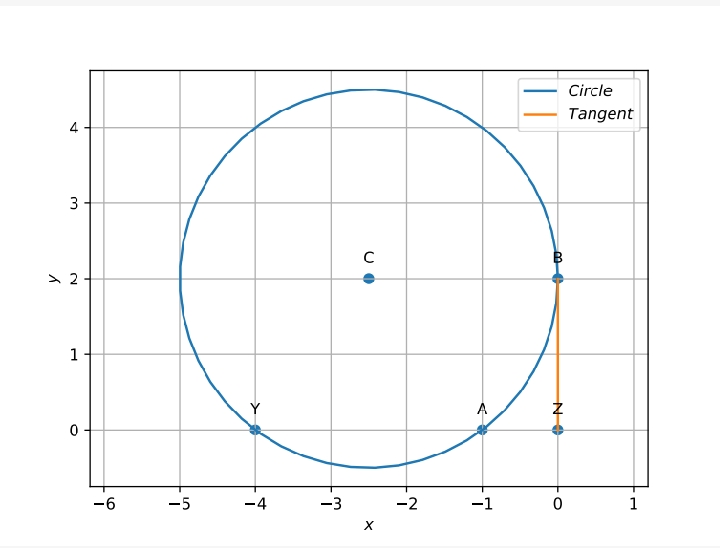
\includegraphics[scale=0.25]{circle1.jpg}
  \section{Software}
  We can plot the cicle with the help of the following code :
 \vspace{3mm} 
\begin{lstlisting}
https://github.com/Gowt-hami/fwc-1-module1/blob/main/par.py
\end{lstlisting}
\end{center}
\end{document}
